\documentclass[11pt,letterpaper]{article}
\PassOptionsToPackage{hyphens}{url}
\usepackage[margin=.83in,top=.8in,bottom=.8in,headheight=15pt]{geometry}
\usepackage[T1]{fontenc}
\usepackage{lmodern,amsmath,amssymb,mathtools,bm,booktabs,array,graphicx,tikz}
\usetikzlibrary{arrows.meta,positioning,calc,decorations.pathreplacing,patterns}
\definecolor{ink}{HTML}{17344D}\definecolor{accent}{HTML}{087E8B}\definecolor{pale}{HTML}{EDF5F5}\definecolor{gold}{HTML}{AD6B19}
\providecommand{\dd}{\,\mathrm{d}}\providecommand{\R}{\mathbb{R}}
\providecommand{\E}{\mathbb{E}}\providecommand{\Var}{\operatorname{Var}}
\providecommand{\Cov}{\operatorname{Cov}}\providecommand{\diag}{\operatorname{diag}}
\providecommand{\norm}[1]{\left\lVert#1\right\rVert}
\providecommand{\abs}[1]{\left|#1\right|}
\usepackage{microtype,hyperref,fancyhdr,enumitem,amsthm,sectsty,needspace}
\allsectionsfont{\raggedright}
\hypersetup{colorlinks=true,linkcolor=ink,urlcolor=accent,pdfauthor={Zan Ahmad},pdftitle={Logistic regression and a neural-network classifier / Lecture notes}}
\setlength{\parindent}{0pt}\setlength{\parskip}{6pt}\linespread{1.07}
\setlist{itemsep=3pt,topsep=4pt,leftmargin=*}
\emergencystretch=2em\clubpenalty=10000\widowpenalty=10000
\pagestyle{fancy}\fancyhf{}\fancyhead[L]{\small Scientific Computing in Python}\fancyhead[R]{\small Lecture 6}
\fancyfoot[L]{\footnotesize Zan Ahmad}\fancyfoot[R]{\footnotesize\thepage}\renewcommand{\headrulewidth}{.3pt}
\newtheorem{proposition}{Proposition}\newtheorem{theorem}{Theorem}\newtheorem{lemma}{Lemma}
\theoremstyle{definition}\newtheorem{definition}{Definition}\newtheorem{example}{Example}
\numberwithin{equation}{section}
\begin{document}
{\small\scshape Scientific Computing in Python\hfill Lecture 6}\par\medskip
{\raggedright\hyphenpenalty=10000\exhyphenpenalty=10000\LARGE\bfseries\color{ink} Logistic regression and a neural-network classifier\par}\medskip
{\small Lecture notes}\par\bigskip
A binary classifier maps a vector of measured features to a score and then applies a decision threshold. We begin with logistic regression and derive its loss gradient. A small neural network replaces the linear feature map by a nonlinear one. The models are compared on the same held-out observations, after their training choices have been fixed.

\section{Logistic scores}
\hypertarget{note-logistic-scores}{}\label{note:logistic-scores}
{\small \href{slides.html\#frame=logistic-scores\&step=1}{Slides for this section}}\par
Let $x_i\in\R^d$ and $y_i\in\{0,1\}$. Logistic regression forms an affine score $a_i=x_i^{\mathsf T}w+b$ and maps it to $(0,1)$ using the sigmoid. The inverse relation is the log odds. At threshold one half, the decision boundary is the hyperplane $x^{\mathsf T}w+b=0$.

\[
p_i=\sigma(a_i)=\frac1{1+e^{-a_i}},\qquad a_i=x_i^{\mathsf T}w+b.
\]

\[
\log\frac{p_i}{1-p_i}=a_i.
\]

\subsection*{Threshold geometry}
\[
p_i\geq\frac12\iff a_i\geq0.
\]

Changing the threshold changes the decision rule. It does not change the fitted score surface.
\section{Bernoulli negative log likelihood}
\hypertarget{note-bernoulli-negative-log-likelihood}{}\label{note:bernoulli-negative-log-likelihood}
{\small \href{slides.html\#frame=bernoulli-negative-log-likelihood\&step=1}{Slides for this section}}\par
Assuming conditionally independent labels under the fitted model gives a product of Bernoulli probabilities. Taking minus the logarithm produces a sum. Expressing the loss in terms of logits yields a stable computational form using logaddexp.

\[
\ell_i=-y_i\log p_i-(1-y_i)\log(1-p_i)
=\log(1+e^{a_i})-y_ia_i.
\]

\begin{minipage}{\linewidth}
\begin{verbatim}
loss = np.mean(np.logaddexp(0, logits)-y*logits)
\end{verbatim}
\end{minipage}

\subsection*{The logit derivative}
\[
\frac{\partial\ell_i}{\partial a_i}=\sigma(a_i)-y_i=p_i-y_i.
\]

\[
\nabla_wL=\frac1nX^{\mathsf T}(p-y).
\]
This simple residual drives the parameter update.
\section{Gradient descent and regularization}
\hypertarget{note-gradient-descent-and-regularization}{}\label{note:gradient-descent-and-regularization}
{\small \href{slides.html\#frame=gradient-descent-and-regularization\&step=1}{Slides for this section}}\par
A gradient step moves opposite the derivative of the objective. Adding a squared weight penalty discourages large coefficients and changes the gradient. The step size controls the numerical optimization and must be distinguished from statistical regularization. A decreasing training loss alone does not demonstrate good prediction on new observations.

\[
L(w,b)=\frac1n\sum_i\ell_i+\frac\lambda2\|w\|_2^2.
\]

\[
w\leftarrow w-\eta\left[\frac1nX^{\mathsf T}(p-y)+\lambda w\right].
\]

\subsection*{Intercept update}
With no penalty on the intercept,
\[
b\leftarrow b-\eta\frac1n\sum_i(p_i-y_i).
\]

The choice of which parameters receive a penalty belongs to the objective definition.
\begin{center}\begin{minipage}{.98\linewidth}\centering
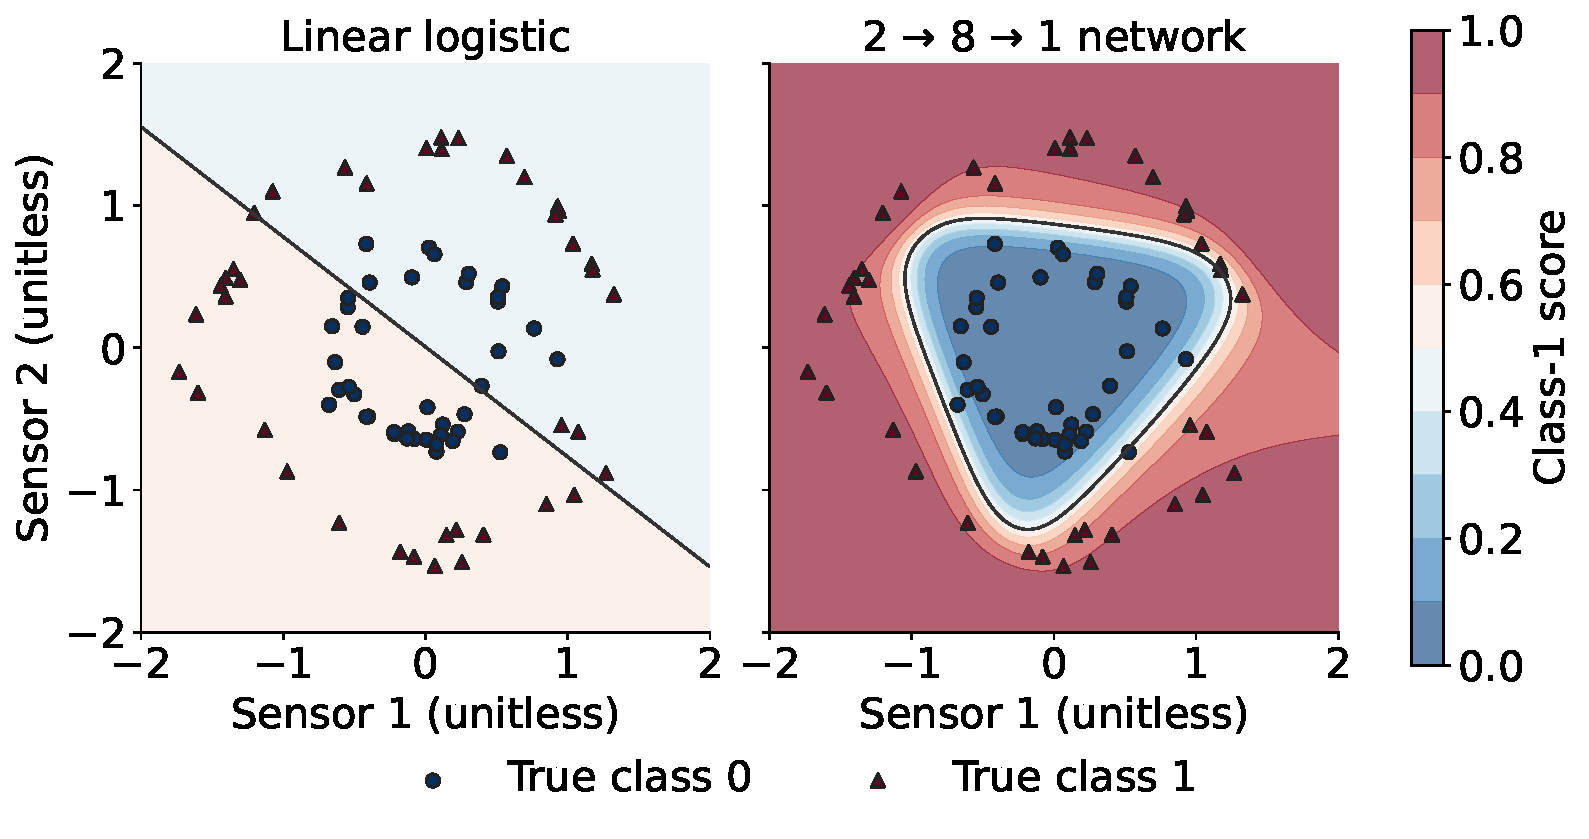
\includegraphics[width=.96\linewidth,height=.57\textheight,keepaspectratio]{decision-comparison.pdf}\par\smallskip
{\small Both frozen models use the same training subset and scaling. Points are held-out examples, backgrounds are class-one scores and dark curves mark the one-half threshold. A separate marker key identifies true classes: circles for class 0 and triangles for class 1.}
\end{minipage}\end{center}
\section{A nonlinear hidden layer}
\hypertarget{note-a-nonlinear-hidden-layer}{}\label{note:a-nonlinear-hidden-layer}
{\small \href{slides.html\#frame=linear-and-nonlinear-decision-boundaries-figure\&step=1}{Slides for this section}}\par
For $X\in\R^{n\times d}$, choose $W_1\in\R^{d\times h}$ and a row bias $b_1\in\R^h$. Applying tanh entrywise gives $H\in\R^{n\times h}$. A second affine map produces one logit per row. The nonlinearity allows curved decision boundaries; without it, two affine maps collapse to one.

\[
H=\tanh(XW_1+b_1),\qquad a=Hw_2+b_2,\qquad p=\sigma(a).
\]

Shapes: $(n\times d)(d\times h)=n\times h$, then $(n\times h)(h\times1)=n\times1$.

\subsection*{Backpropagation through tanh}
Let $D=(p-y)/n$. Then
\[
\nabla_{w_2}L=H^{\mathsf T}D,
\quad
D_1=(Dw_2^{\mathsf T})\odot(1-H^2).
\]

\[
\nabla_{W_1}L=X^{\mathsf T}D_1.
\]
Weight-penalty derivatives are added separately.
\Needspace{10\baselineskip}
\section{Confusion counts}
\hypertarget{note-confusion-counts}{}\label{note:confusion-counts}
{\small \href{slides.html\#frame=confusion-counts\&step=1}{Slides for this section}}\par
A confusion matrix records counts after thresholding scores. Rows denote actual classes and columns predicted classes in this course. Accuracy combines correct decisions; precision conditions on positive predictions; recall conditions on actual positives. Empty denominators require an explicit convention rather than an unreported numerical replacement.

\[
\mathrm{accuracy}=\frac{TP+TN}{N},\quad
\mathrm{precision}=\frac{TP}{TP+FP},\quad
\mathrm{recall}=\frac{TP}{TP+FN}.
\]

Each denominator specifies a different reference group.

\subsection*{A worked confusion matrix}
\[
\begin{array}{c|cc}&\widehat y=0&\widehat y=1\\\hline y=0&30&10\\y=1&5&35\end{array}
\]

Accuracy $=65/80$, precision $=35/45$, recall $=35/40$. This illustrative matrix is separate from the companion's computed result.
\begin{center}\begin{minipage}{.98\linewidth}\centering
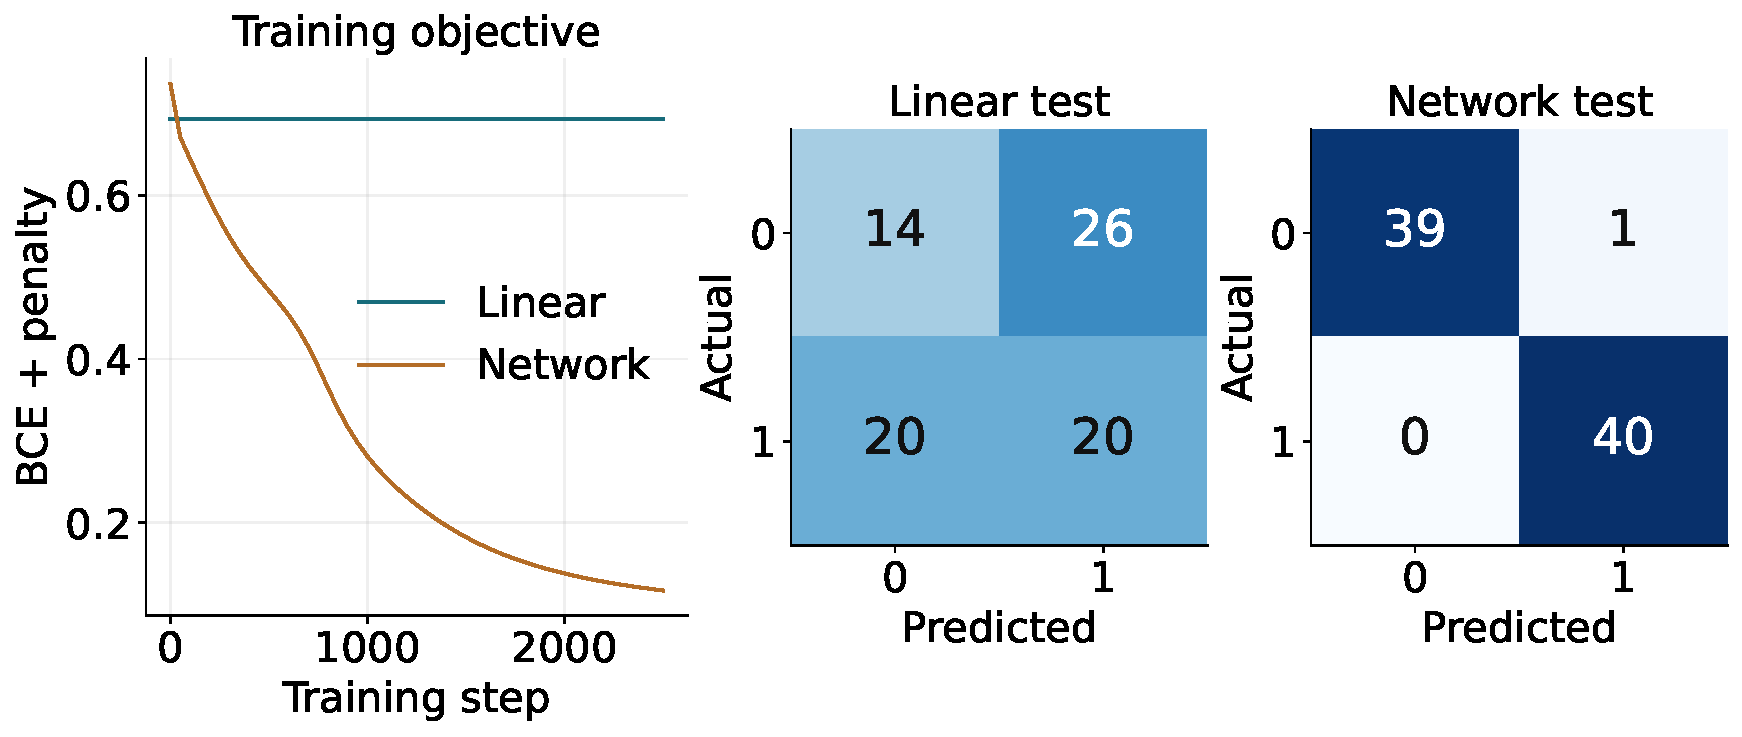
\includegraphics[width=.96\linewidth,height=.57\textheight,keepaspectratio]{loss-and-confusion.pdf}\par\smallskip
{\small Training loss includes the stated weight penalty; confusion matrices use actual classes as rows and predicted classes as columns. Each test class contains 40 examples.}
\end{minipage}\end{center}
\section{A controlled model comparison}
\hypertarget{note-a-controlled-model-comparison}{}\label{note:a-controlled-model-comparison}
{\small \href{slides.html\#frame=training-loss-and-held-out-counts-figure\&step=1}{Slides for this section}}\par
The same train/test split and training-derived standardization are used for both models. Decisions about architecture, penalties, training duration, and threshold precede reading the test outcome. Repeatedly choosing settings from test accuracy converts the test set into a tuning set. Synthetic success applies to the generator used and cannot establish clinical performance.

Both classifiers receive the same feature representation and the same training rows.

The held-out comparison measures the consequences of the fitted functions, not differences in which test observations were selected.

\subsection*{Reproducibility and variability}
A fixed seed reproduces one random split and initialization.

It does not quantify variation over other samples. Repeated, properly separated experiments are needed to study that variation.
\bigskip
\section*{Exercises}
\par\noindent\begin{minipage}{\linewidth}
\subsection*{H6-1. Read a confusion matrix}
For a new classifier, TN =\allowbreak{} 36, FP =\allowbreak{} 4, FN =\allowbreak{} 9 and TP =\allowbreak{} 11. New practice; 10 feedback points.

\textbf{a} Write the 2-by-2 matrix with actual classes as rows, give the total sample count and calculate accuracy.

\end{minipage}\par\medskip
\textbf{b} Calculate precision and recall for class one and explain their denominators.

\textbf{c} Would always predicting class zero attain high accuracy here, and what would it miss?

\par\noindent\begin{minipage}{\linewidth}
\subsection*{H6-2. A threshold is a decision rule}
Scores are [0.2, 0.4, 0.6, 0.8] and actual labels are [0, 1, 0, 1]. Predict one when score is at least the threshold. New practice; 10 feedback points.

\textbf{a} At threshold 0.5, give predicted labels and TN, FP, FN, TP.

\end{minipage}\par\medskip
\textbf{b} At threshold 0.4, give accuracy, precision and recall.

\textbf{c} If these were final test data, could selecting 0.4 because of this result support a fresh unbiased test claim?

\par\noindent\begin{minipage}{\linewidth}
\subsection*{H6-3. Trace a forward pass}
Use the lesson network with two inputs, eight hidden tanh units and one output score. New practice; 10 feedback points.

\textbf{a} For a batch of five examples, state the shapes of X, W1, hidden values, W2 and output scores, and count the trainable numbers.

\end{minipage}\par\medskip
\textbf{b} In a separate two-hidden-unit illustration, hidden values are [0.5, -0.25], output weights [2, -4] and output bias -1. Find the logit and the label at threshold 0.5; sigmoid(1) is approximately 0.731.

\textbf{c} Explain what happens to the possible decision boundary if every hidden tanh is replaced by the identity function.

\par\noindent\begin{minipage}{\linewidth}
\subsection*{H6-4. Audit a comparison claim}
A report standardizes all data, tries ten network widths, keeps the best test score and claims that neural networks are always necessary for the ring problem. New practice; 10 feedback points.

\textbf{a} Identify two distinct ways held-out information entered the reported workflow.

\end{minipage}\par\medskip
\textbf{b} Describe a corrected sequence for a final comparison.

\textbf{c} Explain how the radius-based comparator limits the claim that a neural network is necessary.

\section*{References}
\noindent\begin{minipage}{\linewidth}
Original Python Lecture 5. PDF pages 5--6.

\url{https://zanahmad.com/files/scientific-python/Lecture_5__Intro_to_Python.pdf}
\end{minipage}\par\medskip
\noindent\begin{minipage}{\linewidth}
scikit-learn supervised neural-network guide. Sections 1.17.1 and 1.17.5--1.17.7: MLP, mathematical formulation and scaling.

\url{https://scikit-learn.org/stable/modules/neural_networks_supervised.html}
\end{minipage}\par\medskip
\noindent\begin{minipage}{\linewidth}
scikit-learn model-evaluation guide. Binary classification metrics: confusion counts, precision and recall.

\url{https://scikit-learn.org/stable/modules/model_evaluation.html}
\end{minipage}\par\medskip
\noindent\begin{minipage}{\linewidth}
scikit-learn common pitfalls. Sections 12.1--12.2.1: consistent preprocessing and training-only fitting.

\url{https://scikit-learn.org/stable/common_pitfalls.html#data-leakage}
\end{minipage}\par\medskip
Python source materials: Phillip Kerger (2023). Course adaptation and additional exposition: Zan Ahmad.

\end{document}
